\documentclass{article}\usepackage[]{graphicx}\usepackage[]{color}
% maxwidth is the original width if it is less than linewidth
% otherwise use linewidth (to make sure the graphics do not exceed the margin)
\makeatletter
\def\maxwidth{ %
  \ifdim\Gin@nat@width>\linewidth
    \linewidth
  \else
    \Gin@nat@width
  \fi
}
\makeatother

\definecolor{fgcolor}{rgb}{0.345, 0.345, 0.345}
\newcommand{\hlnum}[1]{\textcolor[rgb]{0.686,0.059,0.569}{#1}}%
\newcommand{\hlstr}[1]{\textcolor[rgb]{0.192,0.494,0.8}{#1}}%
\newcommand{\hlcom}[1]{\textcolor[rgb]{0.678,0.584,0.686}{\textit{#1}}}%
\newcommand{\hlopt}[1]{\textcolor[rgb]{0,0,0}{#1}}%
\newcommand{\hlstd}[1]{\textcolor[rgb]{0.345,0.345,0.345}{#1}}%
\newcommand{\hlkwa}[1]{\textcolor[rgb]{0.161,0.373,0.58}{\textbf{#1}}}%
\newcommand{\hlkwb}[1]{\textcolor[rgb]{0.69,0.353,0.396}{#1}}%
\newcommand{\hlkwc}[1]{\textcolor[rgb]{0.333,0.667,0.333}{#1}}%
\newcommand{\hlkwd}[1]{\textcolor[rgb]{0.737,0.353,0.396}{\textbf{#1}}}%
\let\hlipl\hlkwb

\usepackage{framed}
\makeatletter
\newenvironment{kframe}{%
 \def\at@end@of@kframe{}%
 \ifinner\ifhmode%
  \def\at@end@of@kframe{\end{minipage}}%
  \begin{minipage}{\columnwidth}%
 \fi\fi%
 \def\FrameCommand##1{\hskip\@totalleftmargin \hskip-\fboxsep
 \colorbox{shadecolor}{##1}\hskip-\fboxsep
     % There is no \\@totalrightmargin, so:
     \hskip-\linewidth \hskip-\@totalleftmargin \hskip\columnwidth}%
 \MakeFramed {\advance\hsize-\width
   \@totalleftmargin\z@ \linewidth\hsize
   \@setminipage}}%
 {\par\unskip\endMakeFramed%
 \at@end@of@kframe}
\makeatother

\definecolor{shadecolor}{rgb}{.97, .97, .97}
\definecolor{messagecolor}{rgb}{0, 0, 0}
\definecolor{warningcolor}{rgb}{1, 0, 1}
\definecolor{errorcolor}{rgb}{1, 0, 0}
\newenvironment{knitrout}{}{} % an empty environment to be redefined in TeX

\usepackage{alltt}

\usepackage{float}

% Set the margins on the page to not be so large
\addtolength{\oddsidemargin}{-.875in}
\addtolength{\evensidemargin}{-.875in}
\addtolength{\textwidth}{1.75in}
\addtolength{\topmargin}{-.875in}
\addtolength{\textheight}{1.75in}

% Take off page numbering
\pagenumbering{gobble}
\IfFileExists{upquote.sty}{\usepackage{upquote}}{}
\begin{document}

\title{%
  2.2.1: R - Residual Diagnostics\\
  \smallskip
  \large Stat 5100: Dr. Bean
}
\date{}

\maketitle

\textbf{Example: } (The Toluca Company data from Handout \#2)

\begin{knitrout}
\definecolor{shadecolor}{rgb}{0.969, 0.969, 0.969}\color{fgcolor}\begin{kframe}
\begin{alltt}
\hlcom{# Input same toluca data from Ch. 1}
\hlkwd{library}\hlstd{(stat5100)}
\hlkwd{data}\hlstd{(toluca)}

\hlcom{# Fit a simple linear model with Y=workhours and X=lotsize}
\hlstd{toluca_lm} \hlkwb{<-} \hlkwd{lm}\hlstd{(workhours} \hlopt{~} \hlstd{lotsize,} \hlkwc{data} \hlstd{= toluca)}
\hlstd{toluca_lm}
\end{alltt}
\begin{verbatim}
## 
## Call:
## lm(formula = workhours ~ lotsize, data = toluca)
## 
## Coefficients:
## (Intercept)      lotsize  
##       62.37         3.57
\end{verbatim}
\begin{alltt}
\hlcom{# Look at a sequence plot to evaluate independence}
\hlkwd{seq_plot}\hlstd{(toluca_lm)}
\end{alltt}
\end{kframe}
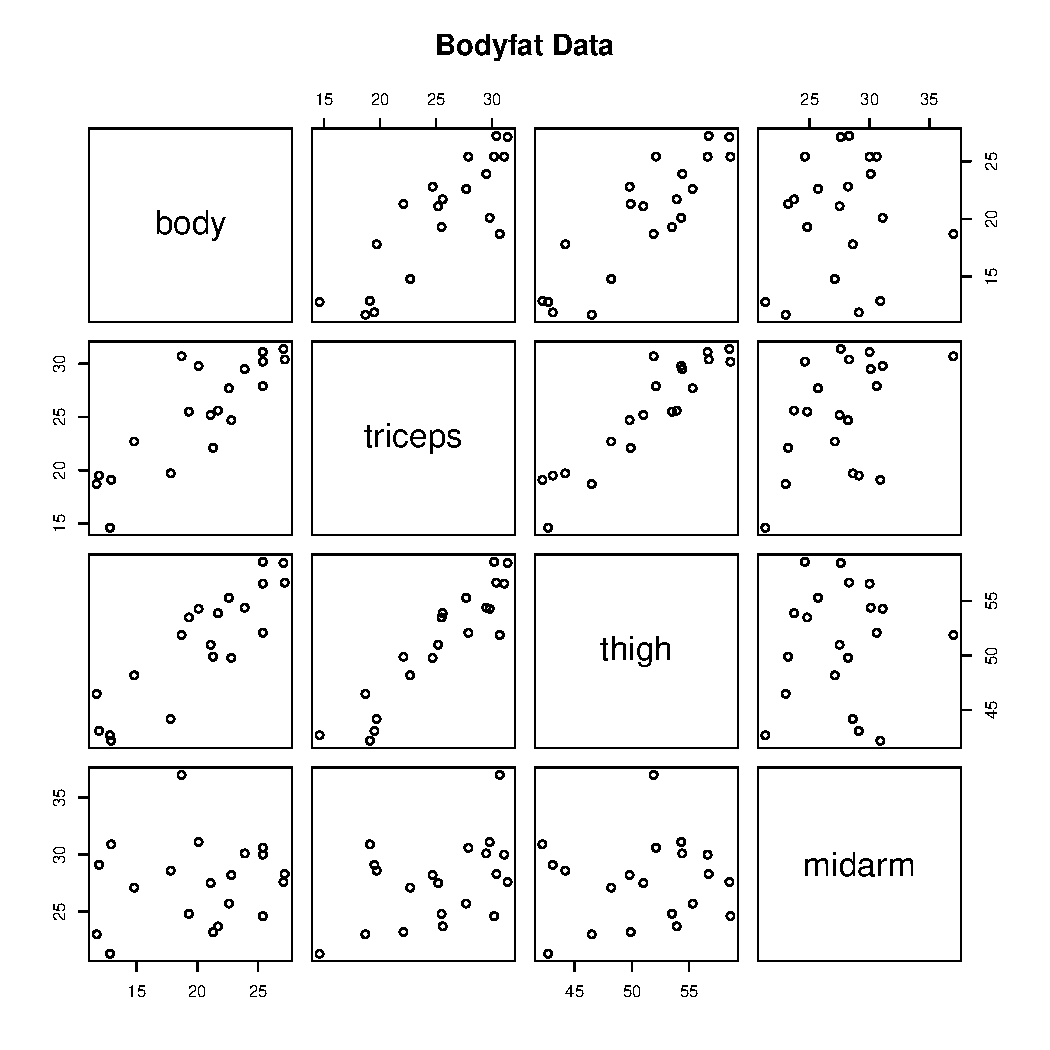
\includegraphics[width=0.6\textwidth]{figure/unnamed-chunk-1-1} 
\begin{kframe}\begin{alltt}
\hlcom{# Numerical Diagnostics}

\hlcom{# Perform F-test for lack of fit.}
\hlkwd{ftest_lackfit_lm}\hlstd{(toluca_lm)}
\end{alltt}
\begin{verbatim}
## Analysis of Variance Table
## 
## Model 1: workhours ~ lotsize
## Model 2: workhours ~ lotsize
##   Res.Df   RSS Df Sum of Sq      F Pr(>F)
## 1     23 54825                           
## 2     14 37581  9     17245 0.7138 0.6893
\end{verbatim}
\begin{alltt}
\hlcom{# Brown-Forsythe test for constant variance}
\hlkwd{brown_forsythe_lm}\hlstd{(toluca_lm)}
\end{alltt}
\begin{verbatim}
## [1] "Brown-forsythe test for constant variance in the residuals:"
## [1] "T-statistic: 1.3165, p-value: 0.201"
\end{verbatim}
\begin{alltt}
\hlcom{# Correlation test of normality}
\hlkwd{cor_normality_lm}\hlstd{(toluca_lm)}
\end{alltt}
\begin{verbatim}
## Correlation test of normality:
##                   resid expected_norm
## resid         1.0000000     0.9915055
## expected_norm 0.9915055     1.0000000
## 
## Total observations: 25
## Make sure to consult with table B.6 for your final result.
\end{verbatim}
\end{kframe}
\end{knitrout}


\end{document}
